\documentclass[1p]{elsarticle_modified}
%\bibliographystyle{elsarticle-num}

%\usepackage[colorlinks]{hyperref}
%\usepackage{abbrmath_seonhwa} %\Abb, \Ascr, \Acal ,\Abf, \Afrak
\usepackage{amsfonts}
\usepackage{amssymb}
\usepackage{amsmath}
\usepackage{amsthm}
\usepackage{scalefnt}
\usepackage{amsbsy}
\usepackage{kotex}
\usepackage{caption}
\usepackage{subfig}
\usepackage{color}
\usepackage{graphicx}
\usepackage{xcolor} %% white, black, red, green, blue, cyan, magenta, yellow
\usepackage{float}
\usepackage{setspace}
\usepackage{hyperref}

\usepackage{tikz}
\usetikzlibrary{arrows}

\usepackage{multirow}
\usepackage{array} % fixed length table
\usepackage{hhline}

%%%%%%%%%%%%%%%%%%%%%
\makeatletter
\renewcommand*\env@matrix[1][\arraystretch]{%
	\edef\arraystretch{#1}%
	\hskip -\arraycolsep
	\let\@ifnextchar\new@ifnextchar
	\array{*\c@MaxMatrixCols c}}
\makeatother %https://tex.stackexchange.com/questions/14071/how-can-i-increase-the-line-spacing-in-a-matrix
%%%%%%%%%%%%%%%

\usepackage[normalem]{ulem}

\newcommand{\msout}[1]{\ifmmode\text{\sout{\ensuremath{#1}}}\else\sout{#1}\fi}
%SOURCE: \msout is \stkout macro in https://tex.stackexchange.com/questions/20609/strikeout-in-math-mode

\newcommand{\cancel}[1]{
	\ifmmode
	{\color{red}\msout{#1}}
	\else
	{\color{red}\sout{#1}}
	\fi
}

\newcommand{\add}[1]{
	{\color{blue}\uwave{#1}}
}

\newcommand{\replace}[2]{
	\ifmmode
	{\color{red}\msout{#1}}{\color{blue}\uwave{#2}}
	\else
	{\color{red}\sout{#1}}{\color{blue}\uwave{#2}}
	\fi
}

\newcommand{\Sol}{\mathcal{S}} %segment
\newcommand{\D}{D} %diagram
\newcommand{\A}{\mathcal{A}} %arc


%%%%%%%%%%%%%%%%%%%%%%%%%%%%%5 test

\def\sl{\operatorname{\textup{SL}}(2,\Cbb)}
\def\psl{\operatorname{\textup{PSL}}(2,\Cbb)}
\def\quan{\mkern 1mu \triangleright \mkern 1mu}

\theoremstyle{definition}
\newtheorem{thm}{Theorem}[section]
\newtheorem{prop}[thm]{Proposition}
\newtheorem{lem}[thm]{Lemma}
\newtheorem{ques}[thm]{Question}
\newtheorem{cor}[thm]{Corollary}
\newtheorem{defn}[thm]{Definition}
\newtheorem{exam}[thm]{Example}
\newtheorem{rmk}[thm]{Remark}
\newtheorem{alg}[thm]{Algorithm}

\newcommand{\I}{\sqrt{-1}}
\begin{document}

%\begin{frontmatter}
%
%\title{Boundary parabolic representations of knots up to 8 crossings}
%
%%% Group authors per affiliation:
%\author{Yunhi Cho} 
%\address{Department of Mathematics, University of Seoul, Seoul, Korea}
%\ead{yhcho@uos.ac.kr}
%
%
%\author{Seonhwa Kim} %\fnref{s_kim}}
%\address{Center for Geometry and Physics, Institute for Basic Science, Pohang, 37673, Korea}
%\ead{ryeona17@ibs.re.kr}
%
%\author{Hyuk Kim}
%\address{Department of Mathematical Sciences, Seoul National University, Seoul 08826, Korea}
%\ead{hyukkim@snu.ac.kr}
%
%\author{Seokbeom Yoon}
%\address{Department of Mathematical Sciences, Seoul National University, Seoul, 08826,  Korea}
%\ead{sbyoon15@snu.ac.kr}
%
%\begin{abstract}
%We find all boundary parabolic representation of knots up to 8 crossings.
%
%\end{abstract}
%\begin{keyword}
%    \MSC[2010] 57M25 
%\end{keyword}
%
%\end{frontmatter}

%\linenumbers
%\tableofcontents
%
\newcommand\colored[1]{\textcolor{white}{\rule[-0.35ex]{0.8em}{1.4ex}}\kern-0.8em\color{red} #1}%
%\newcommand\colored[1]{\textcolor{white}{ #1}\kern-2.17ex	\textcolor{white}{ #1}\kern-1.81ex	\textcolor{white}{ #1}\kern-2.15ex\color{red}#1	}

{\Large $\underline{12a_{0766}~(K12a_{0766})}$}

\setlength{\tabcolsep}{10pt}
\renewcommand{\arraystretch}{1.6}
\vspace{1cm}\begin{tabular}{m{100pt}>{\centering\arraybackslash}m{274pt}}
\multirow{5}{120pt}{
	\centering
	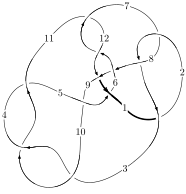
\includegraphics[width=112pt]{../../../GIT/diagram.site/Diagrams/png/1567_12a_0766.png}\\
\ \ \ A knot diagram\footnotemark}&
\allowdisplaybreaks
\textbf{Linearized knot diagam} \\
\cline{2-2}
 &
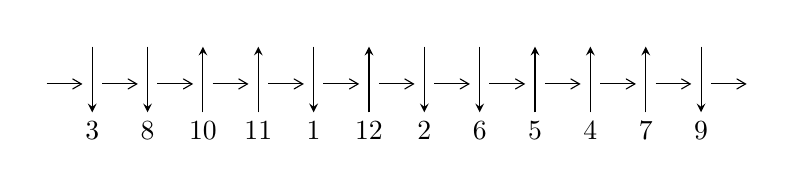
\begin{tikzpicture}[x=20pt, y=17pt]
	% nodes
	\node (C0) at (0, 0) {};
	\node (C1) at (1, 0) {};
	\node (C1U) at (1, +1) {};
	\node (C1D) at (1, -1) {3};

	\node (C2) at (2, 0) {};
	\node (C2U) at (2, +1) {};
	\node (C2D) at (2, -1) {8};

	\node (C3) at (3, 0) {};
	\node (C3U) at (3, +1) {};
	\node (C3D) at (3, -1) {10};

	\node (C4) at (4, 0) {};
	\node (C4U) at (4, +1) {};
	\node (C4D) at (4, -1) {11};

	\node (C5) at (5, 0) {};
	\node (C5U) at (5, +1) {};
	\node (C5D) at (5, -1) {1};

	\node (C6) at (6, 0) {};
	\node (C6U) at (6, +1) {};
	\node (C6D) at (6, -1) {12};

	\node (C7) at (7, 0) {};
	\node (C7U) at (7, +1) {};
	\node (C7D) at (7, -1) {2};

	\node (C8) at (8, 0) {};
	\node (C8U) at (8, +1) {};
	\node (C8D) at (8, -1) {6};

	\node (C9) at (9, 0) {};
	\node (C9U) at (9, +1) {};
	\node (C9D) at (9, -1) {5};

	\node (C10) at (10, 0) {};
	\node (C10U) at (10, +1) {};
	\node (C10D) at (10, -1) {4};

	\node (C11) at (11, 0) {};
	\node (C11U) at (11, +1) {};
	\node (C11D) at (11, -1) {7};

	\node (C12) at (12, 0) {};
	\node (C12U) at (12, +1) {};
	\node (C12D) at (12, -1) {9};
	\node (C13) at (13, 0) {};

	% arrows
	\draw[->,>={angle 60}]
	(C0) edge (C1) (C1) edge (C2) (C2) edge (C3) (C3) edge (C4) (C4) edge (C5) (C5) edge (C6) (C6) edge (C7) (C7) edge (C8) (C8) edge (C9) (C9) edge (C10) (C10) edge (C11) (C11) edge (C12) (C12) edge (C13) ;	\draw[->,>=stealth]
	(C1U) edge (C1D) (C2U) edge (C2D) (C3D) edge (C3U) (C4D) edge (C4U) (C5U) edge (C5D) (C6D) edge (C6U) (C7U) edge (C7D) (C8U) edge (C8D) (C9D) edge (C9U) (C10D) edge (C10U) (C11D) edge (C11U) (C12U) edge (C12D) ;
	\end{tikzpicture} \\
\hhline{~~} \\& 
\textbf{Solving Sequence} \\ \cline{2-2} 
 &
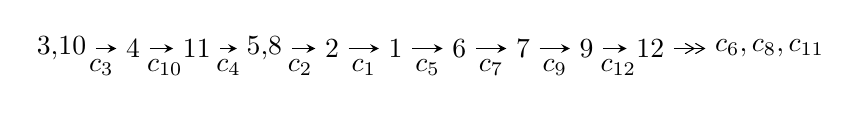
\begin{tikzpicture}[x=23pt, y=7pt]
	% node
	\node (A0) at (-1/8, 0) {3,10};
	\node (A1) at (1, 0) {4};
	\node (A2) at (2, 0) {11};
	\node (A3) at (49/16, 0) {5,8};
	\node (A4) at (33/8, 0) {2};
	\node (A5) at (41/8, 0) {1};
	\node (A6) at (49/8, 0) {6};
	\node (A7) at (57/8, 0) {7};
	\node (A8) at (65/8, 0) {9};
	\node (A9) at (73/8, 0) {12};
	\node (C1) at (1/2, -1) {$c_{3}$};
	\node (C2) at (3/2, -1) {$c_{10}$};
	\node (C3) at (5/2, -1) {$c_{4}$};
	\node (C4) at (29/8, -1) {$c_{2}$};
	\node (C5) at (37/8, -1) {$c_{1}$};
	\node (C6) at (45/8, -1) {$c_{5}$};
	\node (C7) at (53/8, -1) {$c_{7}$};
	\node (C8) at (61/8, -1) {$c_{9}$};
	\node (C9) at (69/8, -1) {$c_{12}$};
	\node (A10) at (11, 0) {$c_{6},c_{8},c_{11}$};

	% edge
	\draw[->,>=stealth]	
	(A0) edge (A1) (A1) edge (A2) (A2) edge (A3) (A3) edge (A4) (A4) edge (A5) (A5) edge (A6) (A6) edge (A7) (A7) edge (A8) (A8) edge (A9) ;
	\draw[->>,>={angle 60}]	
	(A9) edge (A10);
\end{tikzpicture} \\ 

\end{tabular} \\

\footnotetext{
The image of knot diagram is generated by the software ``\textbf{Draw programme}" developed by Andrew Bartholomew(\url{http://www.layer8.co.uk/maths/draw/index.htm\#Running-draw}), where we modified some parts for our purpose(\url{https://github.com/CATsTAILs/LinksPainter}).
}\phantom \\ \newline 
\centering \textbf{Ideals for irreducible components\footnotemark of $X_{\text{par}}$} 
 
\begin{align*}
I^u_{1}&=\langle 
2.13361\times10^{216} u^{128}-2.24626\times10^{216} u^{127}+\cdots+5.09830\times10^{216} b+8.25708\times10^{217},\\
\phantom{I^u_{1}}&\phantom{= \langle  }-5.76761\times10^{217} u^{128}+1.76555\times10^{218} u^{127}+\cdots+2.19227\times10^{218} a-3.76892\times10^{218},\\
\phantom{I^u_{1}}&\phantom{= \langle  }u^{129}-57 u^{127}+\cdots+378 u+43\rangle \\
I^u_{2}&=\langle 
2 u^{22}-20 u^{20}+\cdots-7 u^2+b,\;-3 u^{23}-3 u^{22}+\cdots+a+4,\;u^{24}-12 u^{22}+\cdots-2 u+1\rangle \\
I^u_{3}&=\langle 
b+1,\;a+1,\;u+1\rangle \\
\\
\end{align*}
\raggedright * 3 irreducible components of $\dim_{\mathbb{C}}=0$, with total 154 representations.\\
\footnotetext{All coefficients of polynomials are rational numbers. But the coefficients are sometimes approximated in decimal forms when there is not enough margin.}
\newpage
\renewcommand{\arraystretch}{1}
\centering \section*{I. $I^u_{1}= \langle 2.13\times10^{216} u^{128}-2.25\times10^{216} u^{127}+\cdots+5.10\times10^{216} b+8.26\times10^{217},\;-5.77\times10^{217} u^{128}+1.77\times10^{218} u^{127}+\cdots+2.19\times10^{218} a-3.77\times10^{218},\;u^{129}-57 u^{127}+\cdots+378 u+43 \rangle$}
\flushleft \textbf{(i) Arc colorings}\\
\begin{tabular}{m{7pt} m{180pt} m{7pt} m{180pt} }
\flushright $a_{3}=$&$\begin{pmatrix}1\\0\end{pmatrix}$ \\
\flushright $a_{10}=$&$\begin{pmatrix}0\\u\end{pmatrix}$ \\
\flushright $a_{4}=$&$\begin{pmatrix}1\\- u^2\end{pmatrix}$ \\
\flushright $a_{11}=$&$\begin{pmatrix}u\\- u^3+u\end{pmatrix}$ \\
\flushright $a_{5}=$&$\begin{pmatrix}- u^2+1\\u^4-2 u^2\end{pmatrix}$ \\
\flushright $a_{8}=$&$\begin{pmatrix}0.263089 u^{128}-0.805353 u^{127}+\cdots+42.7132 u+1.71919\\-0.418495 u^{128}+0.440590 u^{127}+\cdots-138.953 u-16.1957\end{pmatrix}$ \\
\flushright $a_{2}=$&$\begin{pmatrix}0.467938 u^{128}-0.812760 u^{127}+\cdots+28.7148 u+7.66234\\-0.705149 u^{128}+0.785581 u^{127}+\cdots-30.0980 u-6.28193\end{pmatrix}$ \\
\flushright $a_{1}=$&$\begin{pmatrix}-0.237211 u^{128}-0.0271790 u^{127}+\cdots-1.38322 u+1.38042\\-0.705149 u^{128}+0.785581 u^{127}+\cdots-30.0980 u-6.28193\end{pmatrix}$ \\
\flushright $a_{6}=$&$\begin{pmatrix}0.755620 u^{128}-0.177142 u^{127}+\cdots+47.3681 u+1.03645\\-0.0305009 u^{128}-0.0755006 u^{127}+\cdots-2.33441 u+1.39110\end{pmatrix}$ \\
\flushright $a_{7}=$&$\begin{pmatrix}-0.0733243 u^{128}-0.511720 u^{127}+\cdots+60.5543 u+8.77827\\0.587856 u^{128}-0.0941282 u^{127}+\cdots+75.5430 u+9.18933\end{pmatrix}$ \\
\flushright $a_{9}=$&$\begin{pmatrix}- u^5+2 u^3- u\\u^7-3 u^5+2 u^3+u\end{pmatrix}$ \\
\flushright $a_{12}=$&$\begin{pmatrix}0.448679 u^{128}-0.802998 u^{127}+\cdots+8.13708 u+4.46535\\-0.545577 u^{128}+0.686006 u^{127}+\cdots-3.01559 u-2.16240\end{pmatrix}$\\&\end{tabular}
\flushleft \textbf{(ii) Obstruction class $= -1$}\\~\\
\flushleft \textbf{(iii) Cusp Shapes $= -0.688840 u^{128}-1.19440 u^{127}+\cdots-15.5285 u-16.6790$}\\~\\
\newpage\renewcommand{\arraystretch}{1}
\flushleft \textbf{(iv) u-Polynomials at the component}\newline \\
\begin{tabular}{m{50pt}|m{274pt}}
Crossings & \hspace{64pt}u-Polynomials at each crossing \\
\hline $$\begin{aligned}c_{1}\end{aligned}$$&$\begin{aligned}
&u^{129}+58 u^{128}+\cdots+1112505 u+85849
\end{aligned}$\\
\hline $$\begin{aligned}c_{2},c_{7}\end{aligned}$$&$\begin{aligned}
&u^{129}-29 u^{127}+\cdots+259 u+293
\end{aligned}$\\
\hline $$\begin{aligned}c_{3},c_{4},c_{10}\end{aligned}$$&$\begin{aligned}
&u^{129}-57 u^{127}+\cdots+378 u+43
\end{aligned}$\\
\hline $$\begin{aligned}c_{5}\end{aligned}$$&$\begin{aligned}
&u^{129}+3 u^{128}+\cdots-40 u+1
\end{aligned}$\\
\hline $$\begin{aligned}c_{6},c_{11}\end{aligned}$$&$\begin{aligned}
&u^{129}+u^{128}+\cdots+76623 u+52995
\end{aligned}$\\
\hline $$\begin{aligned}c_{8}\end{aligned}$$&$\begin{aligned}
&u^{129}-9 u^{128}+\cdots-40 u+1
\end{aligned}$\\
\hline $$\begin{aligned}c_{9}\end{aligned}$$&$\begin{aligned}
&u^{129}-3 u^{128}+\cdots+20927496 u+1128105
\end{aligned}$\\
\hline $$\begin{aligned}c_{12}\end{aligned}$$&$\begin{aligned}
&u^{129}+4 u^{128}+\cdots-146894 u-14831
\end{aligned}$\\
\hline
\end{tabular}\\~\\
\newpage\renewcommand{\arraystretch}{1}
\flushleft \textbf{(v) Riley Polynomials at the component}\newline \\
\begin{tabular}{m{50pt}|m{274pt}}
Crossings & \hspace{64pt}Riley Polynomials at each crossing \\
\hline $$\begin{aligned}c_{1}\end{aligned}$$&$\begin{aligned}
&y^{129}+38 y^{128}+\cdots+16755519645 y-7370050801
\end{aligned}$\\
\hline $$\begin{aligned}c_{2},c_{7}\end{aligned}$$&$\begin{aligned}
&y^{129}-58 y^{128}+\cdots+1112505 y-85849
\end{aligned}$\\
\hline $$\begin{aligned}c_{3},c_{4},c_{10}\end{aligned}$$&$\begin{aligned}
&y^{129}-114 y^{128}+\cdots-32126 y-1849
\end{aligned}$\\
\hline $$\begin{aligned}c_{5}\end{aligned}$$&$\begin{aligned}
&y^{129}-5 y^{128}+\cdots+90 y-1
\end{aligned}$\\
\hline $$\begin{aligned}c_{6},c_{11}\end{aligned}$$&$\begin{aligned}
&y^{129}+89 y^{128}+\cdots-89198342211 y-2808470025
\end{aligned}$\\
\hline $$\begin{aligned}c_{8}\end{aligned}$$&$\begin{aligned}
&y^{129}-13 y^{128}+\cdots+10 y-1
\end{aligned}$\\
\hline $$\begin{aligned}c_{9}\end{aligned}$$&$\begin{aligned}
&y^{129}+41 y^{128}+\cdots+17191577913966 y-1272620891025
\end{aligned}$\\
\hline $$\begin{aligned}c_{12}\end{aligned}$$&$\begin{aligned}
&y^{129}-34 y^{128}+\cdots+16675400862 y-219958561
\end{aligned}$\\
\hline
\end{tabular}\\~\\
\newpage\flushleft \textbf{(vi) Complex Volumes and Cusp Shapes}
$$\begin{array}{c|c|c}  
\text{Solutions to }I^u_{1}& \I (\text{vol} + \sqrt{-1}CS) & \text{Cusp shape}\\
 \hline 
\begin{aligned}
u &= -0.949751 + 0.312486 I \\
a &= -0.245150 - 1.217980 I \\
b &= -0.053229 + 0.489319 I\end{aligned}
 & -1.37418 - 3.62180 I & \phantom{-0.000000 } 0 \\ \hline\begin{aligned}
u &= -0.949751 - 0.312486 I \\
a &= -0.245150 + 1.217980 I \\
b &= -0.053229 - 0.489319 I\end{aligned}
 & -1.37418 + 3.62180 I & \phantom{-0.000000 } 0 \\ \hline\begin{aligned}
u &= \phantom{-}0.381049 + 0.913700 I \\
a &= -0.512439 - 1.315800 I \\
b &= -1.031630 + 0.528294 I\end{aligned}
 & -5.02675 + 4.64385 I & \phantom{-0.000000 } 0 \\ \hline\begin{aligned}
u &= \phantom{-}0.381049 - 0.913700 I \\
a &= -0.512439 + 1.315800 I \\
b &= -1.031630 - 0.528294 I\end{aligned}
 & -5.02675 - 4.64385 I & \phantom{-0.000000 } 0 \\ \hline\begin{aligned}
u &= -0.866089 + 0.420234 I \\
a &= -0.442386 + 1.197430 I \\
b &= -0.333734 - 0.814259 I\end{aligned}
 & -1.03335 + 4.34050 I & \phantom{-0.000000 } 0 \\ \hline\begin{aligned}
u &= -0.866089 - 0.420234 I \\
a &= -0.442386 - 1.197430 I \\
b &= -0.333734 + 0.814259 I\end{aligned}
 & -1.03335 - 4.34050 I & \phantom{-0.000000 } 0 \\ \hline\begin{aligned}
u &= \phantom{-}0.683065 + 0.677856 I \\
a &= -0.361680 - 0.409401 I \\
b &= \phantom{-}1.013710 + 0.399081 I\end{aligned}
 & -3.98667 + 0.69907 I & \phantom{-0.000000 } 0 \\ \hline\begin{aligned}
u &= \phantom{-}0.683065 - 0.677856 I \\
a &= -0.361680 + 0.409401 I \\
b &= \phantom{-}1.013710 - 0.399081 I\end{aligned}
 & -3.98667 - 0.69907 I & \phantom{-0.000000 } 0 \\ \hline\begin{aligned}
u &= -1.012930 + 0.246613 I \\
a &= \phantom{-}0.575278 + 0.469381 I \\
b &= \phantom{-}0.972479 - 0.530189 I\end{aligned}
 & \phantom{-}1.40813 + 4.17445 I & \phantom{-0.000000 } 0 \\ \hline\begin{aligned}
u &= -1.012930 - 0.246613 I \\
a &= \phantom{-}0.575278 - 0.469381 I \\
b &= \phantom{-}0.972479 + 0.530189 I\end{aligned}
 & \phantom{-}1.40813 - 4.17445 I & \phantom{-0.000000 } 0\\
 \hline 
 \end{array}$$\newpage$$\begin{array}{c|c|c}  
\text{Solutions to }I^u_{1}& \I (\text{vol} + \sqrt{-1}CS) & \text{Cusp shape}\\
 \hline 
\begin{aligned}
u &= \phantom{-}0.120180 + 1.042100 I \\
a &= \phantom{-}0.587260 - 0.370386 I \\
b &= \phantom{-}0.951327 + 0.351873 I\end{aligned}
 & -6.36332 - 1.31649 I & \phantom{-0.000000 } 0 \\ \hline\begin{aligned}
u &= \phantom{-}0.120180 - 1.042100 I \\
a &= \phantom{-}0.587260 + 0.370386 I \\
b &= \phantom{-}0.951327 - 0.351873 I\end{aligned}
 & -6.36332 + 1.31649 I & \phantom{-0.000000 } 0 \\ \hline\begin{aligned}
u &= \phantom{-}0.930564 + 0.535062 I \\
a &= \phantom{-}0.232044 + 0.420312 I \\
b &= -1.139950 - 0.597740 I\end{aligned}
 & -3.39947 - 9.60540 I & \phantom{-0.000000 } 0 \\ \hline\begin{aligned}
u &= \phantom{-}0.930564 - 0.535062 I \\
a &= \phantom{-}0.232044 - 0.420312 I \\
b &= -1.139950 + 0.597740 I\end{aligned}
 & -3.39947 + 9.60540 I & \phantom{-0.000000 } 0 \\ \hline\begin{aligned}
u &= \phantom{-}0.258275 + 0.852940 I \\
a &= \phantom{-}1.04567 + 1.25372 I \\
b &= \phantom{-}1.173070 - 0.639730 I\end{aligned}
 & -5.4770 + 14.4708 I & \phantom{-0.000000 } 0 \\ \hline\begin{aligned}
u &= \phantom{-}0.258275 - 0.852940 I \\
a &= \phantom{-}1.04567 - 1.25372 I \\
b &= \phantom{-}1.173070 + 0.639730 I\end{aligned}
 & -5.4770 - 14.4708 I & \phantom{-0.000000 } 0 \\ \hline\begin{aligned}
u &= \phantom{-}1.137320 + 0.022675 I \\
a &= -0.161520 - 0.175917 I \\
b &= \phantom{-}0.596067 + 0.326746 I\end{aligned}
 & \phantom{-}2.31439 + 0.13029 I & \phantom{-0.000000 } 0 \\ \hline\begin{aligned}
u &= \phantom{-}1.137320 - 0.022675 I \\
a &= -0.161520 + 0.175917 I \\
b &= \phantom{-}0.596067 - 0.326746 I\end{aligned}
 & \phantom{-}2.31439 - 0.13029 I & \phantom{-0.000000 } 0 \\ \hline\begin{aligned}
u &= \phantom{-}1.102490 + 0.358833 I \\
a &= \phantom{-}0.052065 + 1.356020 I \\
b &= \phantom{-}1.263830 - 0.200178 I\end{aligned}
 & -6.13755 - 1.11746 I & \phantom{-0.000000 } 0 \\ \hline\begin{aligned}
u &= \phantom{-}1.102490 - 0.358833 I \\
a &= \phantom{-}0.052065 - 1.356020 I \\
b &= \phantom{-}1.263830 + 0.200178 I\end{aligned}
 & -6.13755 + 1.11746 I & \phantom{-0.000000 } 0\\
 \hline 
 \end{array}$$\newpage$$\begin{array}{c|c|c}  
\text{Solutions to }I^u_{1}& \I (\text{vol} + \sqrt{-1}CS) & \text{Cusp shape}\\
 \hline 
\begin{aligned}
u &= -0.246164 + 0.794294 I \\
a &= -0.386614 + 0.196484 I \\
b &= \phantom{-}0.370391 - 0.944177 I\end{aligned}
 & -3.02843 - 8.71041 I & \phantom{-0.000000 } 0 \\ \hline\begin{aligned}
u &= -0.246164 - 0.794294 I \\
a &= -0.386614 - 0.196484 I \\
b &= \phantom{-}0.370391 + 0.944177 I\end{aligned}
 & -3.02843 + 8.71041 I & \phantom{-0.000000 } 0 \\ \hline\begin{aligned}
u &= -0.283413 + 0.756145 I \\
a &= \phantom{-}0.266452 - 0.756504 I \\
b &= -0.452930 + 0.551945 I\end{aligned}
 & -3.38000 - 0.26645 I & \phantom{-0.000000 } 0 \\ \hline\begin{aligned}
u &= -0.283413 - 0.756145 I \\
a &= \phantom{-}0.266452 + 0.756504 I \\
b &= -0.452930 - 0.551945 I\end{aligned}
 & -3.38000 + 0.26645 I & \phantom{-0.000000 } 0 \\ \hline\begin{aligned}
u &= -0.034989 + 0.800453 I \\
a &= \phantom{-}1.36090 - 0.58764 I \\
b &= \phantom{-}0.996535 - 0.319770 I\end{aligned}
 & -6.92317 + 1.00814 I & -12.18026 + 0. I\phantom{ +0.000000I} \\ \hline\begin{aligned}
u &= -0.034989 - 0.800453 I \\
a &= \phantom{-}1.36090 + 0.58764 I \\
b &= \phantom{-}0.996535 + 0.319770 I\end{aligned}
 & -6.92317 - 1.00814 I & -12.18026 + 0. I\phantom{ +0.000000I} \\ \hline\begin{aligned}
u &= \phantom{-}0.126930 + 0.784165 I \\
a &= -1.149040 - 0.097972 I \\
b &= -1.342670 - 0.116692 I\end{aligned}
 & -9.11009 + 5.26813 I & -8.05145 - 5.13781 I \\ \hline\begin{aligned}
u &= \phantom{-}0.126930 - 0.784165 I \\
a &= -1.149040 + 0.097972 I \\
b &= -1.342670 + 0.116692 I\end{aligned}
 & -9.11009 - 5.26813 I & -8.05145 + 5.13781 I \\ \hline\begin{aligned}
u &= -0.187496 + 0.764059 I \\
a &= -1.73126 + 1.16904 I \\
b &= -1.055730 - 0.571772 I\end{aligned}
 & -1.05862 - 8.07165 I & \phantom{-0.000000 -}0. + 8.98454 I \\ \hline\begin{aligned}
u &= -0.187496 - 0.764059 I \\
a &= -1.73126 - 1.16904 I \\
b &= -1.055730 + 0.571772 I\end{aligned}
 & -1.05862 + 8.07165 I & \phantom{-0.000000 } 0. - 8.98454 I\\
 \hline 
 \end{array}$$\newpage$$\begin{array}{c|c|c}  
\text{Solutions to }I^u_{1}& \I (\text{vol} + \sqrt{-1}CS) & \text{Cusp shape}\\
 \hline 
\begin{aligned}
u &= \phantom{-}1.030500 + 0.640829 I \\
a &= -0.216380 - 1.198020 I \\
b &= -1.027760 + 0.456095 I\end{aligned}
 & -3.59587 + 7.09073 I & \phantom{-0.000000 } 0 \\ \hline\begin{aligned}
u &= \phantom{-}1.030500 - 0.640829 I \\
a &= -0.216380 + 1.198020 I \\
b &= -1.027760 - 0.456095 I\end{aligned}
 & -3.59587 - 7.09073 I & \phantom{-0.000000 } 0 \\ \hline\begin{aligned}
u &= -1.220350 + 0.209824 I \\
a &= \phantom{-}0.240259 + 1.184820 I \\
b &= \phantom{-}1.132200 - 0.505673 I\end{aligned}
 & -2.05649 + 2.37182 I & \phantom{-0.000000 } 0 \\ \hline\begin{aligned}
u &= -1.220350 - 0.209824 I \\
a &= \phantom{-}0.240259 - 1.184820 I \\
b &= \phantom{-}1.132200 + 0.505673 I\end{aligned}
 & -2.05649 - 2.37182 I & \phantom{-0.000000 } 0 \\ \hline\begin{aligned}
u &= -1.239870 + 0.079195 I \\
a &= \phantom{-}0.079776 + 0.181516 I \\
b &= -1.308510 + 0.359200 I\end{aligned}
 & -0.76367 + 4.11159 I & \phantom{-0.000000 } 0 \\ \hline\begin{aligned}
u &= -1.239870 - 0.079195 I \\
a &= \phantom{-}0.079776 - 0.181516 I \\
b &= -1.308510 - 0.359200 I\end{aligned}
 & -0.76367 - 4.11159 I & \phantom{-0.000000 } 0 \\ \hline\begin{aligned}
u &= -0.305571 + 0.691387 I \\
a &= \phantom{-}1.31729 - 1.56690 I \\
b &= \phantom{-}0.935225 + 0.280011 I\end{aligned}
 & -3.19789 - 3.11388 I & -6.21792 + 5.42458 I \\ \hline\begin{aligned}
u &= -0.305571 - 0.691387 I \\
a &= \phantom{-}1.31729 + 1.56690 I \\
b &= \phantom{-}0.935225 - 0.280011 I\end{aligned}
 & -3.19789 + 3.11388 I & -6.21792 - 5.42458 I \\ \hline\begin{aligned}
u &= \phantom{-}1.237240 + 0.189888 I \\
a &= -0.121801 - 0.109652 I \\
b &= \phantom{-}0.987710 + 0.333102 I\end{aligned}
 & \phantom{-}2.27384 + 0.38414 I & \phantom{-0.000000 } 0 \\ \hline\begin{aligned}
u &= \phantom{-}1.237240 - 0.189888 I \\
a &= -0.121801 + 0.109652 I \\
b &= \phantom{-}0.987710 - 0.333102 I\end{aligned}
 & \phantom{-}2.27384 - 0.38414 I & \phantom{-0.000000 } 0\\
 \hline 
 \end{array}$$\newpage$$\begin{array}{c|c|c}  
\text{Solutions to }I^u_{1}& \I (\text{vol} + \sqrt{-1}CS) & \text{Cusp shape}\\
 \hline 
\begin{aligned}
u &= \phantom{-}0.235239 + 0.703017 I \\
a &= \phantom{-}0.404597 - 0.343920 I \\
b &= -0.473645 - 0.664736 I\end{aligned}
 & \phantom{-}0.65019 + 3.24933 I & \phantom{-}1.31667 - 4.26581 I \\ \hline\begin{aligned}
u &= \phantom{-}0.235239 - 0.703017 I \\
a &= \phantom{-}0.404597 + 0.343920 I \\
b &= -0.473645 + 0.664736 I\end{aligned}
 & \phantom{-}0.65019 - 3.24933 I & \phantom{-}1.31667 + 4.26581 I \\ \hline\begin{aligned}
u &= -1.233480 + 0.335060 I \\
a &= -0.732802 + 0.658777 I \\
b &= -1.062360 - 0.337000 I\end{aligned}
 & -3.23505 - 5.10584 I & \phantom{-0.000000 } 0 \\ \hline\begin{aligned}
u &= -1.233480 - 0.335060 I \\
a &= -0.732802 - 0.658777 I \\
b &= -1.062360 + 0.337000 I\end{aligned}
 & -3.23505 + 5.10584 I & \phantom{-0.000000 } 0 \\ \hline\begin{aligned}
u &= \phantom{-}0.641954 + 0.273036 I \\
a &= -0.142359 + 0.908731 I \\
b &= \phantom{-}0.640329 - 0.603514 I\end{aligned}
 & \phantom{-}2.32665 + 0.32348 I & \phantom{-}5.25845 - 1.82103 I \\ \hline\begin{aligned}
u &= \phantom{-}0.641954 - 0.273036 I \\
a &= -0.142359 - 0.908731 I \\
b &= \phantom{-}0.640329 + 0.603514 I\end{aligned}
 & \phantom{-}2.32665 - 0.32348 I & \phantom{-}5.25845 + 1.82103 I \\ \hline\begin{aligned}
u &= -1.285400 + 0.213367 I \\
a &= -0.93465 + 2.85309 I \\
b &= -0.934262 - 0.427913 I\end{aligned}
 & \phantom{-}0.654419 - 1.065000 I & \phantom{-0.000000 } 0 \\ \hline\begin{aligned}
u &= -1.285400 - 0.213367 I \\
a &= -0.93465 - 2.85309 I \\
b &= -0.934262 + 0.427913 I\end{aligned}
 & \phantom{-}0.654419 + 1.065000 I & \phantom{-0.000000 } 0 \\ \hline\begin{aligned}
u &= -1.288580 + 0.195899 I \\
a &= \phantom{-}1.43230 - 1.20557 I \\
b &= -0.982426 + 0.963915 I\end{aligned}
 & \phantom{-}3.71266 + 0.80569 I & \phantom{-0.000000 } 0 \\ \hline\begin{aligned}
u &= -1.288580 - 0.195899 I \\
a &= \phantom{-}1.43230 + 1.20557 I \\
b &= -0.982426 - 0.963915 I\end{aligned}
 & \phantom{-}3.71266 - 0.80569 I & \phantom{-0.000000 } 0\\
 \hline 
 \end{array}$$\newpage$$\begin{array}{c|c|c}  
\text{Solutions to }I^u_{1}& \I (\text{vol} + \sqrt{-1}CS) & \text{Cusp shape}\\
 \hline 
\begin{aligned}
u &= \phantom{-}1.285080 + 0.242605 I \\
a &= -0.325908 + 0.834995 I \\
b &= \phantom{-}0.254221 - 0.713807 I\end{aligned}
 & \phantom{-}0.53289 + 2.24449 I & \phantom{-0.000000 } 0 \\ \hline\begin{aligned}
u &= \phantom{-}1.285080 - 0.242605 I \\
a &= -0.325908 - 0.834995 I \\
b &= \phantom{-}0.254221 + 0.713807 I\end{aligned}
 & \phantom{-}0.53289 - 2.24449 I & \phantom{-0.000000 } 0 \\ \hline\begin{aligned}
u &= -1.288460 + 0.230065 I \\
a &= -1.86772 + 1.35606 I \\
b &= \phantom{-}0.605807 - 0.633999 I\end{aligned}
 & \phantom{-}0.45040 - 4.03098 I & \phantom{-0.000000 } 0 \\ \hline\begin{aligned}
u &= -1.288460 - 0.230065 I \\
a &= -1.86772 - 1.35606 I \\
b &= \phantom{-}0.605807 + 0.633999 I\end{aligned}
 & \phantom{-}0.45040 + 4.03098 I & \phantom{-0.000000 } 0 \\ \hline\begin{aligned}
u &= -0.232760 + 0.633710 I \\
a &= \phantom{-}1.50550 - 1.36661 I \\
b &= \phantom{-}1.270070 + 0.569449 I\end{aligned}
 & -3.18629 - 6.33519 I & -3.14862 + 12.03347 I \\ \hline\begin{aligned}
u &= -0.232760 - 0.633710 I \\
a &= \phantom{-}1.50550 + 1.36661 I \\
b &= \phantom{-}1.270070 - 0.569449 I\end{aligned}
 & -3.18629 + 6.33519 I & -3.14862 - 12.03347 I \\ \hline\begin{aligned}
u &= -1.303760 + 0.250568 I \\
a &= \phantom{-}0.42423 - 2.11325 I \\
b &= \phantom{-}1.101360 + 0.686491 I\end{aligned}
 & \phantom{-}2.99432 - 6.05078 I & \phantom{-0.000000 } 0 \\ \hline\begin{aligned}
u &= -1.303760 - 0.250568 I \\
a &= \phantom{-}0.42423 + 2.11325 I \\
b &= \phantom{-}1.101360 - 0.686491 I\end{aligned}
 & \phantom{-}2.99432 + 6.05078 I & \phantom{-0.000000 } 0 \\ \hline\begin{aligned}
u &= \phantom{-}0.051728 + 0.663678 I \\
a &= -1.51687 - 0.44769 I \\
b &= -1.024090 + 0.575987 I\end{aligned}
 & -1.22613 + 2.75786 I & -2.65450 - 2.60934 I \\ \hline\begin{aligned}
u &= \phantom{-}0.051728 - 0.663678 I \\
a &= -1.51687 + 0.44769 I \\
b &= -1.024090 - 0.575987 I\end{aligned}
 & -1.22613 - 2.75786 I & -2.65450 + 2.60934 I\\
 \hline 
 \end{array}$$\newpage$$\begin{array}{c|c|c}  
\text{Solutions to }I^u_{1}& \I (\text{vol} + \sqrt{-1}CS) & \text{Cusp shape}\\
 \hline 
\begin{aligned}
u &= -0.107918 + 0.656610 I \\
a &= -1.25879 + 2.14517 I \\
b &= -1.061850 - 0.537149 I\end{aligned}
 & -5.38016 - 5.47743 I & -9.82084 + 6.44409 I \\ \hline\begin{aligned}
u &= -0.107918 - 0.656610 I \\
a &= -1.25879 - 2.14517 I \\
b &= -1.061850 + 0.537149 I\end{aligned}
 & -5.38016 + 5.47743 I & -9.82084 - 6.44409 I \\ \hline\begin{aligned}
u &= -0.660616 + 0.073556 I \\
a &= \phantom{-}0.618520 - 1.253390 I \\
b &= \phantom{-}0.895989 + 0.597110 I\end{aligned}
 & \phantom{-}1.57071 - 4.30992 I & \phantom{-}4.28889 + 6.85006 I \\ \hline\begin{aligned}
u &= -0.660616 - 0.073556 I \\
a &= \phantom{-}0.618520 + 1.253390 I \\
b &= \phantom{-}0.895989 - 0.597110 I\end{aligned}
 & \phantom{-}1.57071 + 4.30992 I & \phantom{-}4.28889 - 6.85006 I \\ \hline\begin{aligned}
u &= \phantom{-}1.313710 + 0.241466 I \\
a &= -0.780841 - 0.440678 I \\
b &= -1.068580 - 0.182131 I\end{aligned}
 & \phantom{-}1.08249 + 4.90601 I & \phantom{-0.000000 } 0 \\ \hline\begin{aligned}
u &= \phantom{-}1.313710 - 0.241466 I \\
a &= -0.780841 + 0.440678 I \\
b &= -1.068580 + 0.182131 I\end{aligned}
 & \phantom{-}1.08249 - 4.90601 I & \phantom{-0.000000 } 0 \\ \hline\begin{aligned}
u &= \phantom{-}1.289040 + 0.356639 I \\
a &= -0.041263 - 0.873175 I \\
b &= -0.943221 - 0.301307 I\end{aligned}
 & -2.79875 + 3.16373 I & \phantom{-0.000000 } 0 \\ \hline\begin{aligned}
u &= \phantom{-}1.289040 - 0.356639 I \\
a &= -0.041263 + 0.873175 I \\
b &= -0.943221 + 0.301307 I\end{aligned}
 & -2.79875 - 3.16373 I & \phantom{-0.000000 } 0 \\ \hline\begin{aligned}
u &= \phantom{-}1.331160 + 0.228298 I \\
a &= \phantom{-}0.12635 - 2.10173 I \\
b &= -0.783896 + 1.071910 I\end{aligned}
 & \phantom{-}4.30701 + 6.39294 I & \phantom{-0.000000 } 0 \\ \hline\begin{aligned}
u &= \phantom{-}1.331160 - 0.228298 I \\
a &= \phantom{-}0.12635 + 2.10173 I \\
b &= -0.783896 - 1.071910 I\end{aligned}
 & \phantom{-}4.30701 - 6.39294 I & \phantom{-0.000000 } 0\\
 \hline 
 \end{array}$$\newpage$$\begin{array}{c|c|c}  
\text{Solutions to }I^u_{1}& \I (\text{vol} + \sqrt{-1}CS) & \text{Cusp shape}\\
 \hline 
\begin{aligned}
u &= \phantom{-}1.340690 + 0.174728 I \\
a &= -1.074840 - 0.818066 I \\
b &= \phantom{-}0.441055 + 0.970931 I\end{aligned}
 & \phantom{-}4.93415 + 0.07314 I & \phantom{-0.000000 } 0 \\ \hline\begin{aligned}
u &= \phantom{-}1.340690 - 0.174728 I \\
a &= -1.074840 + 0.818066 I \\
b &= \phantom{-}0.441055 - 0.970931 I\end{aligned}
 & \phantom{-}4.93415 - 0.07314 I & \phantom{-0.000000 } 0 \\ \hline\begin{aligned}
u &= \phantom{-}1.347990 + 0.123766 I \\
a &= \phantom{-}2.47858 + 0.55625 I \\
b &= -0.829918 - 0.381993 I\end{aligned}
 & \phantom{-}1.08424 - 2.31644 I & \phantom{-0.000000 } 0 \\ \hline\begin{aligned}
u &= \phantom{-}1.347990 - 0.123766 I \\
a &= \phantom{-}2.47858 - 0.55625 I \\
b &= -0.829918 + 0.381993 I\end{aligned}
 & \phantom{-}1.08424 + 2.31644 I & \phantom{-0.000000 } 0 \\ \hline\begin{aligned}
u &= -1.264160 + 0.488046 I \\
a &= -0.149323 - 0.190707 I \\
b &= -0.827861 + 0.220619 I\end{aligned}
 & -2.13885 - 4.09392 I & \phantom{-0.000000 } 0 \\ \hline\begin{aligned}
u &= -1.264160 - 0.488046 I \\
a &= -0.149323 + 0.190707 I \\
b &= -0.827861 - 0.220619 I\end{aligned}
 & -2.13885 + 4.09392 I & \phantom{-0.000000 } 0 \\ \hline\begin{aligned}
u &= \phantom{-}1.338380 + 0.267903 I \\
a &= -0.30424 + 2.95672 I \\
b &= \phantom{-}1.015670 - 0.585199 I\end{aligned}
 & -0.80604 + 8.84631 I & \phantom{-0.000000 } 0 \\ \hline\begin{aligned}
u &= \phantom{-}1.338380 - 0.267903 I \\
a &= -0.30424 - 2.95672 I \\
b &= \phantom{-}1.015670 + 0.585199 I\end{aligned}
 & -0.80604 - 8.84631 I & \phantom{-0.000000 } 0 \\ \hline\begin{aligned}
u &= -0.014498 + 0.634879 I \\
a &= \phantom{-}0.965550 + 0.059490 I \\
b &= -0.411697 - 0.598157 I\end{aligned}
 & -3.51388 + 0.94620 I & -5.93034 - 0.85000 I \\ \hline\begin{aligned}
u &= -0.014498 - 0.634879 I \\
a &= \phantom{-}0.965550 - 0.059490 I \\
b &= -0.411697 + 0.598157 I\end{aligned}
 & -3.51388 - 0.94620 I & -5.93034 + 0.85000 I\\
 \hline 
 \end{array}$$\newpage$$\begin{array}{c|c|c}  
\text{Solutions to }I^u_{1}& \I (\text{vol} + \sqrt{-1}CS) & \text{Cusp shape}\\
 \hline 
\begin{aligned}
u &= -1.341020 + 0.325292 I \\
a &= -0.319508 - 0.763984 I \\
b &= \phantom{-}1.399080 - 0.055416 I\end{aligned}
 & -4.49309 - 9.26298 I & \phantom{-0.000000 } 0 \\ \hline\begin{aligned}
u &= -1.341020 - 0.325292 I \\
a &= -0.319508 + 0.763984 I \\
b &= \phantom{-}1.399080 + 0.055416 I\end{aligned}
 & -4.49309 + 9.26298 I & \phantom{-0.000000 } 0 \\ \hline\begin{aligned}
u &= -0.046328 + 0.601989 I \\
a &= \phantom{-}3.03271 + 0.58825 I \\
b &= \phantom{-}0.957541 - 0.270349 I\end{aligned}
 & -3.21632 - 1.82438 I & -7.37850 + 2.56071 I \\ \hline\begin{aligned}
u &= -0.046328 - 0.601989 I \\
a &= \phantom{-}3.03271 - 0.58825 I \\
b &= \phantom{-}0.957541 + 0.270349 I\end{aligned}
 & -3.21632 + 1.82438 I & -7.37850 - 2.56071 I \\ \hline\begin{aligned}
u &= -1.383490 + 0.203364 I \\
a &= \phantom{-}0.77665 - 1.26093 I \\
b &= -0.068033 + 0.886656 I\end{aligned}
 & \phantom{-}5.67947 - 3.84340 I & \phantom{-0.000000 } 0 \\ \hline\begin{aligned}
u &= -1.383490 - 0.203364 I \\
a &= \phantom{-}0.77665 + 1.26093 I \\
b &= -0.068033 - 0.886656 I\end{aligned}
 & \phantom{-}5.67947 + 3.84340 I & \phantom{-0.000000 } 0 \\ \hline\begin{aligned}
u &= \phantom{-}0.286197 + 0.523035 I \\
a &= -0.693003 - 0.555111 I \\
b &= -0.343974 + 0.639364 I\end{aligned}
 & \phantom{-}0.27805 + 1.47291 I & \phantom{-}2.31189 - 3.55895 I \\ \hline\begin{aligned}
u &= \phantom{-}0.286197 - 0.523035 I \\
a &= -0.693003 + 0.555111 I \\
b &= -0.343974 - 0.639364 I\end{aligned}
 & \phantom{-}0.27805 - 1.47291 I & \phantom{-}2.31189 + 3.55895 I \\ \hline\begin{aligned}
u &= \phantom{-}1.398270 + 0.126201 I \\
a &= -1.31607 - 0.81801 I \\
b &= \phantom{-}1.055110 + 0.696789 I\end{aligned}
 & \phantom{-}3.72771 - 1.60223 I & \phantom{-0.000000 } 0 \\ \hline\begin{aligned}
u &= \phantom{-}1.398270 - 0.126201 I \\
a &= -1.31607 + 0.81801 I \\
b &= \phantom{-}1.055110 - 0.696789 I\end{aligned}
 & \phantom{-}3.72771 + 1.60223 I & \phantom{-0.000000 } 0\\
 \hline 
 \end{array}$$\newpage$$\begin{array}{c|c|c}  
\text{Solutions to }I^u_{1}& \I (\text{vol} + \sqrt{-1}CS) & \text{Cusp shape}\\
 \hline 
\begin{aligned}
u &= \phantom{-}1.385930 + 0.258089 I \\
a &= \phantom{-}0.08055 - 2.26566 I \\
b &= -1.30652 + 0.64174 I\end{aligned}
 & \phantom{-}1.95632 + 9.61573 I & \phantom{-0.000000 } 0 \\ \hline\begin{aligned}
u &= \phantom{-}1.385930 - 0.258089 I \\
a &= \phantom{-}0.08055 + 2.26566 I \\
b &= -1.30652 - 0.64174 I\end{aligned}
 & \phantom{-}1.95632 - 9.61573 I & \phantom{-0.000000 } 0 \\ \hline\begin{aligned}
u &= \phantom{-}1.376150 + 0.318704 I \\
a &= \phantom{-}0.62793 + 2.22037 I \\
b &= \phantom{-}1.090750 - 0.600637 I\end{aligned}
 & \phantom{-}3.89259 + 11.99520 I & \phantom{-0.000000 } 0 \\ \hline\begin{aligned}
u &= \phantom{-}1.376150 - 0.318704 I \\
a &= \phantom{-}0.62793 - 2.22037 I \\
b &= \phantom{-}1.090750 + 0.600637 I\end{aligned}
 & \phantom{-}3.89259 - 11.99520 I & \phantom{-0.000000 } 0 \\ \hline\begin{aligned}
u &= -1.397690 + 0.206523 I \\
a &= \phantom{-}0.23606 - 1.56090 I \\
b &= \phantom{-}0.382058 + 0.827988 I\end{aligned}
 & \phantom{-}5.64023 - 4.18276 I & \phantom{-0.000000 } 0 \\ \hline\begin{aligned}
u &= -1.397690 - 0.206523 I \\
a &= \phantom{-}0.23606 + 1.56090 I \\
b &= \phantom{-}0.382058 - 0.827988 I\end{aligned}
 & \phantom{-}5.64023 + 4.18276 I & \phantom{-0.000000 } 0 \\ \hline\begin{aligned}
u &= -1.38908 + 0.28476 I \\
a &= -1.119860 + 0.514843 I \\
b &= \phantom{-}0.446373 - 0.753770 I\end{aligned}
 & \phantom{-}5.80637 - 6.84590 I & \phantom{-0.000000 } 0 \\ \hline\begin{aligned}
u &= -1.38908 - 0.28476 I \\
a &= -1.119860 - 0.514843 I \\
b &= \phantom{-}0.446373 + 0.753770 I\end{aligned}
 & \phantom{-}5.80637 + 6.84590 I & \phantom{-0.000000 } 0 \\ \hline\begin{aligned}
u &= \phantom{-}1.42371 + 0.02338 I \\
a &= \phantom{-}0.81141 + 1.82550 I \\
b &= -0.959007 - 0.705674 I\end{aligned}
 & \phantom{-}7.97409 - 4.11261 I & \phantom{-0.000000 } 0 \\ \hline\begin{aligned}
u &= \phantom{-}1.42371 - 0.02338 I \\
a &= \phantom{-}0.81141 - 1.82550 I \\
b &= -0.959007 + 0.705674 I\end{aligned}
 & \phantom{-}7.97409 + 4.11261 I & \phantom{-0.000000 } 0\\
 \hline 
 \end{array}$$\newpage$$\begin{array}{c|c|c}  
\text{Solutions to }I^u_{1}& \I (\text{vol} + \sqrt{-1}CS) & \text{Cusp shape}\\
 \hline 
\begin{aligned}
u &= -1.42793 + 0.07169 I \\
a &= \phantom{-}0.83963 + 1.73453 I \\
b &= -0.708158 - 0.760697 I\end{aligned}
 & \phantom{-}8.71683 - 1.42435 I & \phantom{-0.000000 } 0 \\ \hline\begin{aligned}
u &= -1.42793 - 0.07169 I \\
a &= \phantom{-}0.83963 - 1.73453 I \\
b &= -0.708158 + 0.760697 I\end{aligned}
 & \phantom{-}8.71683 + 1.42435 I & \phantom{-0.000000 } 0 \\ \hline\begin{aligned}
u &= -0.462513 + 0.332703 I \\
a &= \phantom{-}0.380139 + 0.296075 I \\
b &= -1.120650 + 0.546857 I\end{aligned}
 & -2.04857 + 3.24927 I & -1.31395 - 2.13875 I \\ \hline\begin{aligned}
u &= -0.462513 - 0.332703 I \\
a &= \phantom{-}0.380139 - 0.296075 I \\
b &= -1.120650 - 0.546857 I\end{aligned}
 & -2.04857 - 3.24927 I & -1.31395 + 2.13875 I \\ \hline\begin{aligned}
u &= -0.062807 + 0.564581 I \\
a &= \phantom{-}0.447226 - 0.373579 I \\
b &= \phantom{-}0.856584 + 0.981455 I\end{aligned}
 & -0.13828 - 3.48408 I & -4.17456 + 6.37397 I \\ \hline\begin{aligned}
u &= -0.062807 - 0.564581 I \\
a &= \phantom{-}0.447226 + 0.373579 I \\
b &= \phantom{-}0.856584 - 0.981455 I\end{aligned}
 & -0.13828 + 3.48408 I & -4.17456 - 6.37397 I \\ \hline\begin{aligned}
u &= \phantom{-}1.40597 + 0.32561 I \\
a &= \phantom{-}1.11586 + 1.04697 I \\
b &= -0.417371 - 0.998080 I\end{aligned}
 & \phantom{-}2.22103 + 12.76300 I & \phantom{-0.000000 } 0 \\ \hline\begin{aligned}
u &= \phantom{-}1.40597 - 0.32561 I \\
a &= \phantom{-}1.11586 - 1.04697 I \\
b &= -0.417371 + 0.998080 I\end{aligned}
 & \phantom{-}2.22103 - 12.76300 I & \phantom{-0.000000 } 0 \\ \hline\begin{aligned}
u &= \phantom{-}1.42730 + 0.29068 I \\
a &= -0.23713 - 1.95978 I \\
b &= -0.989534 + 0.413380 I\end{aligned}
 & \phantom{-}2.35464 + 6.74741 I & \phantom{-0.000000 } 0 \\ \hline\begin{aligned}
u &= \phantom{-}1.42730 - 0.29068 I \\
a &= -0.23713 + 1.95978 I \\
b &= -0.989534 - 0.413380 I\end{aligned}
 & \phantom{-}2.35464 - 6.74741 I & \phantom{-0.000000 } 0\\
 \hline 
 \end{array}$$\newpage$$\begin{array}{c|c|c}  
\text{Solutions to }I^u_{1}& \I (\text{vol} + \sqrt{-1}CS) & \text{Cusp shape}\\
 \hline 
\begin{aligned}
u &= \phantom{-}1.42268 + 0.33037 I \\
a &= -0.933547 - 1.033410 I \\
b &= \phantom{-}0.591135 + 0.709360 I\end{aligned}
 & \phantom{-}2.07597 + 4.27513 I & \phantom{-0.000000 } 0 \\ \hline\begin{aligned}
u &= \phantom{-}1.42268 - 0.33037 I \\
a &= -0.933547 + 1.033410 I \\
b &= \phantom{-}0.591135 - 0.709360 I\end{aligned}
 & \phantom{-}2.07597 - 4.27513 I & \phantom{-0.000000 } 0 \\ \hline\begin{aligned}
u &= -1.42028 + 0.35130 I \\
a &= -0.13660 + 2.23521 I \\
b &= -1.181510 - 0.674850 I\end{aligned}
 & -0.1426 - 18.8140 I & \phantom{-0.000000 } 0 \\ \hline\begin{aligned}
u &= -1.42028 - 0.35130 I \\
a &= -0.13660 - 2.23521 I \\
b &= -1.181510 + 0.674850 I\end{aligned}
 & -0.1426 + 18.8140 I & \phantom{-0.000000 } 0 \\ \hline\begin{aligned}
u &= \phantom{-}0.283349 + 0.453426 I \\
a &= -0.833098 - 0.166446 I \\
b &= \phantom{-}0.027745 + 0.713970 I\end{aligned}
 & \phantom{-}0.451489 + 1.313460 I & \phantom{-}4.43011 - 5.18918 I \\ \hline\begin{aligned}
u &= \phantom{-}0.283349 - 0.453426 I \\
a &= -0.833098 + 0.166446 I \\
b &= \phantom{-}0.027745 - 0.713970 I\end{aligned}
 & \phantom{-}0.451489 - 1.313460 I & \phantom{-}4.43011 + 5.18918 I \\ \hline\begin{aligned}
u &= \phantom{-}1.49176 + 0.01117 I \\
a &= -0.40095 + 1.69312 I \\
b &= \phantom{-}0.605739 - 0.736610 I\end{aligned}
 & \phantom{-}6.66225 - 3.55941 I & \phantom{-0.000000 } 0 \\ \hline\begin{aligned}
u &= \phantom{-}1.49176 - 0.01117 I \\
a &= -0.40095 - 1.69312 I \\
b &= \phantom{-}0.605739 + 0.736610 I\end{aligned}
 & \phantom{-}6.66225 + 3.55941 I & \phantom{-0.000000 } 0 \\ \hline\begin{aligned}
u &= -1.45922 + 0.38895 I \\
a &= -0.04132 - 1.98850 I \\
b &= \phantom{-}1.021220 + 0.619356 I\end{aligned}
 & \phantom{-}0.78262 - 9.39430 I & \phantom{-0.000000 } 0 \\ \hline\begin{aligned}
u &= -1.45922 - 0.38895 I \\
a &= -0.04132 + 1.98850 I \\
b &= \phantom{-}1.021220 - 0.619356 I\end{aligned}
 & \phantom{-}0.78262 + 9.39430 I & \phantom{-0.000000 } 0\\
 \hline 
 \end{array}$$\newpage$$\begin{array}{c|c|c}  
\text{Solutions to }I^u_{1}& \I (\text{vol} + \sqrt{-1}CS) & \text{Cusp shape}\\
 \hline 
\begin{aligned}
u &= -1.49938 + 0.21106 I \\
a &= \phantom{-}1.182780 - 0.621147 I \\
b &= -0.852786 + 0.326083 I\end{aligned}
 & \phantom{-}3.02808 - 3.76961 I & \phantom{-0.000000 } 0 \\ \hline\begin{aligned}
u &= -1.49938 - 0.21106 I \\
a &= \phantom{-}1.182780 + 0.621147 I \\
b &= -0.852786 - 0.326083 I\end{aligned}
 & \phantom{-}3.02808 + 3.76961 I & \phantom{-0.000000 } 0 \\ \hline\begin{aligned}
u &= -0.471922\phantom{ +0.000000I} \\
a &= -0.923633\phantom{ +0.000000I} \\
b &= -0.896592\phantom{ +0.000000I}\end{aligned}
 & -1.83682\phantom{ +0.000000I} & -3.53830\phantom{ +0.000000I} \\ \hline\begin{aligned}
u &= -0.211913 + 0.419594 I \\
a &= -0.149374 + 1.219750 I \\
b &= -0.542353 + 0.689988 I\end{aligned}
 & \phantom{-}0.15758 + 2.13562 I & \phantom{-}0.765701 - 1.016074 I \\ \hline\begin{aligned}
u &= -0.211913 - 0.419594 I \\
a &= -0.149374 - 1.219750 I \\
b &= -0.542353 - 0.689988 I\end{aligned}
 & \phantom{-}0.15758 - 2.13562 I & \phantom{-}0.765701 + 1.016074 I \\ \hline\begin{aligned}
u &= -1.54866 + 0.03684 I \\
a &= -0.87285 - 1.46188 I \\
b &= \phantom{-}1.013370 + 0.617331 I\end{aligned}
 & \phantom{-}5.42233 - 8.72251 I & \phantom{-0.000000 } 0 \\ \hline\begin{aligned}
u &= -1.54866 - 0.03684 I \\
a &= -0.87285 + 1.46188 I \\
b &= \phantom{-}1.013370 - 0.617331 I\end{aligned}
 & \phantom{-}5.42233 + 8.72251 I & \phantom{-0.000000 } 0 \\ \hline\begin{aligned}
u &= -0.171390 + 0.265251 I \\
a &= -3.61939 - 1.83440 I \\
b &= \phantom{-}1.024380 - 0.332569 I\end{aligned}
 & -3.72652 + 3.87879 I & -6.37269 - 2.76527 I \\ \hline\begin{aligned}
u &= -0.171390 - 0.265251 I \\
a &= -3.61939 + 1.83440 I \\
b &= \phantom{-}1.024380 + 0.332569 I\end{aligned}
 & -3.72652 - 3.87879 I & -6.37269 + 2.76527 I\\
 \hline 
 \end{array}$$\newpage\newpage\renewcommand{\arraystretch}{1}
\centering \section*{II. $I^u_{2}= \langle 2 u^{22}-20 u^{20}+\cdots-7 u^2+b,\;-3 u^{23}-3 u^{22}+\cdots+a+4,\;u^{24}-12 u^{22}+\cdots-2 u+1 \rangle$}
\flushleft \textbf{(i) Arc colorings}\\
\begin{tabular}{m{7pt} m{180pt} m{7pt} m{180pt} }
\flushright $a_{3}=$&$\begin{pmatrix}1\\0\end{pmatrix}$ \\
\flushright $a_{10}=$&$\begin{pmatrix}0\\u\end{pmatrix}$ \\
\flushright $a_{4}=$&$\begin{pmatrix}1\\- u^2\end{pmatrix}$ \\
\flushright $a_{11}=$&$\begin{pmatrix}u\\- u^3+u\end{pmatrix}$ \\
\flushright $a_{5}=$&$\begin{pmatrix}- u^2+1\\u^4-2 u^2\end{pmatrix}$ \\
\flushright $a_{8}=$&$\begin{pmatrix}3 u^{23}+3 u^{22}+\cdots+3 u-4\\-2 u^{22}+20 u^{20}+\cdots-6 u^3+7 u^2\end{pmatrix}$ \\
\flushright $a_{2}=$&$\begin{pmatrix}- u^{23}+10 u^{21}+\cdots- u^2+6 u\\3 u^{23}-32 u^{21}+\cdots+2 u-1\end{pmatrix}$ \\
\flushright $a_{1}=$&$\begin{pmatrix}2 u^{23}-22 u^{21}+\cdots+8 u-1\\3 u^{23}-32 u^{21}+\cdots+2 u-1\end{pmatrix}$ \\
\flushright $a_{6}=$&$\begin{pmatrix}2 u^{22}+u^{21}+\cdots-2 u-2\\u^{22}-11 u^{20}+\cdots- u-1\end{pmatrix}$ \\
\flushright $a_{7}=$&$\begin{pmatrix}u^{22}+u^{21}+\cdots-2 u-3\\- u^{23}- u^{22}+\cdots-2 u-1\end{pmatrix}$ \\
\flushright $a_{9}=$&$\begin{pmatrix}- u^5+2 u^3- u\\u^7-3 u^5+2 u^3+u\end{pmatrix}$ \\
\flushright $a_{12}=$&$\begin{pmatrix}u^{23}-12 u^{21}+\cdots+7 u-1\\3 u^{23}-32 u^{21}+\cdots+3 u-1\end{pmatrix}$\\&\end{tabular}
\flushleft \textbf{(ii) Obstruction class $= 1$}\\~\\
\flushleft \textbf{(iii) Cusp Shapes $= -5 u^{23}-2 u^{22}+52 u^{21}+13 u^{20}-228 u^{19}-26 u^{18}+527 u^{17}-5 u^{16}-631 u^{15}+75 u^{14}+232 u^{13}-36 u^{12}+296 u^{11}-150 u^{10}-345 u^9+229 u^8+105 u^7-104 u^6-33 u^5+16 u^4+36 u^3-22 u^2-4 u+4$}\\~\\
\newpage\renewcommand{\arraystretch}{1}
\flushleft \textbf{(iv) u-Polynomials at the component}\newline \\
\begin{tabular}{m{50pt}|m{274pt}}
Crossings & \hspace{64pt}u-Polynomials at each crossing \\
\hline $$\begin{aligned}c_{1}\end{aligned}$$&$\begin{aligned}
&u^{24}-12 u^{23}+\cdots-15 u+1
\end{aligned}$\\
\hline $$\begin{aligned}c_{2}\end{aligned}$$&$\begin{aligned}
&u^{24}-6 u^{22}+\cdots+u+1
\end{aligned}$\\
\hline $$\begin{aligned}c_{3},c_{4}\end{aligned}$$&$\begin{aligned}
&u^{24}-12 u^{22}+\cdots-2 u+1
\end{aligned}$\\
\hline $$\begin{aligned}c_{5}\end{aligned}$$&$\begin{aligned}
&u^{24}- u^{23}+\cdots+2 u^3+1
\end{aligned}$\\
\hline $$\begin{aligned}c_{6}\end{aligned}$$&$\begin{aligned}
&u^{24}+10 u^{22}+\cdots- u+1
\end{aligned}$\\
\hline $$\begin{aligned}c_{7}\end{aligned}$$&$\begin{aligned}
&u^{24}-6 u^{22}+\cdots- u+1
\end{aligned}$\\
\hline $$\begin{aligned}c_{8}\end{aligned}$$&$\begin{aligned}
&u^{24}+3 u^{23}+\cdots-2 u^2+1
\end{aligned}$\\
\hline $$\begin{aligned}c_{9}\end{aligned}$$&$\begin{aligned}
&u^{24}+4 u^{22}+\cdots+2 u+1
\end{aligned}$\\
\hline $$\begin{aligned}c_{10}\end{aligned}$$&$\begin{aligned}
&u^{24}-12 u^{22}+\cdots+2 u+1
\end{aligned}$\\
\hline $$\begin{aligned}c_{11}\end{aligned}$$&$\begin{aligned}
&u^{24}+10 u^{22}+\cdots+u+1
\end{aligned}$\\
\hline $$\begin{aligned}c_{12}\end{aligned}$$&$\begin{aligned}
&u^{24}-4 u^{23}+\cdots-6 u^2+1
\end{aligned}$\\
\hline
\end{tabular}\\~\\
\newpage\renewcommand{\arraystretch}{1}
\flushleft \textbf{(v) Riley Polynomials at the component}\newline \\
\begin{tabular}{m{50pt}|m{274pt}}
Crossings & \hspace{64pt}Riley Polynomials at each crossing \\
\hline $$\begin{aligned}c_{1}\end{aligned}$$&$\begin{aligned}
&y^{24}+12 y^{23}+\cdots+5 y+1
\end{aligned}$\\
\hline $$\begin{aligned}c_{2},c_{7}\end{aligned}$$&$\begin{aligned}
&y^{24}-12 y^{23}+\cdots-15 y+1
\end{aligned}$\\
\hline $$\begin{aligned}c_{3},c_{4},c_{10}\end{aligned}$$&$\begin{aligned}
&y^{24}-24 y^{23}+\cdots+12 y+1
\end{aligned}$\\
\hline $$\begin{aligned}c_{5}\end{aligned}$$&$\begin{aligned}
&y^{24}-7 y^{23}+\cdots-4 y^2+1
\end{aligned}$\\
\hline $$\begin{aligned}c_{6},c_{11}\end{aligned}$$&$\begin{aligned}
&y^{24}+20 y^{23}+\cdots+21 y+1
\end{aligned}$\\
\hline $$\begin{aligned}c_{8}\end{aligned}$$&$\begin{aligned}
&y^{24}-3 y^{23}+\cdots-4 y+1
\end{aligned}$\\
\hline $$\begin{aligned}c_{9}\end{aligned}$$&$\begin{aligned}
&y^{24}+8 y^{23}+\cdots+8 y+1
\end{aligned}$\\
\hline $$\begin{aligned}c_{12}\end{aligned}$$&$\begin{aligned}
&y^{24}-12 y^{23}+\cdots-12 y+1
\end{aligned}$\\
\hline
\end{tabular}\\~\\
\newpage\flushleft \textbf{(vi) Complex Volumes and Cusp Shapes}
$$\begin{array}{c|c|c}  
\text{Solutions to }I^u_{2}& \I (\text{vol} + \sqrt{-1}CS) & \text{Cusp shape}\\
 \hline 
\begin{aligned}
u &= -0.068651 + 0.929424 I \\
a &= -0.779468 - 0.069325 I \\
b &= -0.919955 + 0.342426 I\end{aligned}
 & -5.90696 + 1.40699 I & -0.05401 - 5.04118 I \\ \hline\begin{aligned}
u &= -0.068651 - 0.929424 I \\
a &= -0.779468 + 0.069325 I \\
b &= -0.919955 - 0.342426 I\end{aligned}
 & -5.90696 - 1.40699 I & -0.05401 + 5.04118 I \\ \hline\begin{aligned}
u &= -1.169690 + 0.336481 I \\
a &= \phantom{-}0.118835 - 0.515687 I \\
b &= \phantom{-}1.023000 + 0.327982 I\end{aligned}
 & -2.71990 - 5.96107 I & -2.03566 + 9.01778 I \\ \hline\begin{aligned}
u &= -1.169690 - 0.336481 I \\
a &= \phantom{-}0.118835 + 0.515687 I \\
b &= \phantom{-}1.023000 - 0.327982 I\end{aligned}
 & -2.71990 + 5.96107 I & -2.03566 - 9.01778 I \\ \hline\begin{aligned}
u &= -1.216630 + 0.130232 I \\
a &= -0.817041 - 0.399318 I \\
b &= -1.160540 + 0.376595 I\end{aligned}
 & -1.09013 + 3.04838 I & -1.88313 - 2.66207 I \\ \hline\begin{aligned}
u &= -1.216630 - 0.130232 I \\
a &= -0.817041 + 0.399318 I \\
b &= -1.160540 - 0.376595 I\end{aligned}
 & -1.09013 - 3.04838 I & -1.88313 + 2.66207 I \\ \hline\begin{aligned}
u &= \phantom{-}1.249520 + 0.073520 I \\
a &= \phantom{-}1.42032 + 0.82987 I \\
b &= -0.649867 + 0.185310 I\end{aligned}
 & \phantom{-}1.068270 - 0.560706 I & -1.91586 + 1.84291 I \\ \hline\begin{aligned}
u &= \phantom{-}1.249520 - 0.073520 I \\
a &= \phantom{-}1.42032 - 0.82987 I \\
b &= -0.649867 - 0.185310 I\end{aligned}
 & \phantom{-}1.068270 + 0.560706 I & -1.91586 - 1.84291 I \\ \hline\begin{aligned}
u &= \phantom{-}1.231740 + 0.410206 I \\
a &= \phantom{-}0.463258 + 0.212630 I \\
b &= \phantom{-}0.838774 + 0.283314 I\end{aligned}
 & -1.97455 + 3.43328 I & \phantom{-}0.001801 + 0.732890 I \\ \hline\begin{aligned}
u &= \phantom{-}1.231740 - 0.410206 I \\
a &= \phantom{-}0.463258 - 0.212630 I \\
b &= \phantom{-}0.838774 - 0.283314 I\end{aligned}
 & -1.97455 - 3.43328 I & \phantom{-}0.001801 - 0.732890 I\\
 \hline 
 \end{array}$$\newpage$$\begin{array}{c|c|c}  
\text{Solutions to }I^u_{2}& \I (\text{vol} + \sqrt{-1}CS) & \text{Cusp shape}\\
 \hline 
\begin{aligned}
u &= -0.324470 + 0.572839 I \\
a &= \phantom{-}0.78856 - 2.18880 I \\
b &= \phantom{-}1.095880 + 0.468311 I\end{aligned}
 & -3.77922 - 5.20044 I & -5.17463 + 7.04376 I \\ \hline\begin{aligned}
u &= -0.324470 - 0.572839 I \\
a &= \phantom{-}0.78856 + 2.18880 I \\
b &= \phantom{-}1.095880 - 0.468311 I\end{aligned}
 & -3.77922 + 5.20044 I & -5.17463 - 7.04376 I \\ \hline\begin{aligned}
u &= \phantom{-}1.335640 + 0.131798 I \\
a &= -1.49295 - 0.94299 I \\
b &= \phantom{-}0.927331 + 0.901413 I\end{aligned}
 & \phantom{-}4.76519 - 1.46228 I & \phantom{-}8.75844 + 4.53633 I \\ \hline\begin{aligned}
u &= \phantom{-}1.335640 - 0.131798 I \\
a &= -1.49295 + 0.94299 I \\
b &= \phantom{-}0.927331 - 0.901413 I\end{aligned}
 & \phantom{-}4.76519 + 1.46228 I & \phantom{-}8.75844 - 4.53633 I \\ \hline\begin{aligned}
u &= -1.382630 + 0.158548 I \\
a &= \phantom{-}0.06907 - 1.77420 I \\
b &= \phantom{-}0.706472 + 0.869930 I\end{aligned}
 & \phantom{-}5.39705 - 5.11184 I & \phantom{-}5.06340 + 6.86539 I \\ \hline\begin{aligned}
u &= -1.382630 - 0.158548 I \\
a &= \phantom{-}0.06907 + 1.77420 I \\
b &= \phantom{-}0.706472 - 0.869930 I\end{aligned}
 & \phantom{-}5.39705 + 5.11184 I & \phantom{-}5.06340 - 6.86539 I \\ \hline\begin{aligned}
u &= \phantom{-}1.41196 + 0.28189 I \\
a &= \phantom{-}0.12280 - 2.23498 I \\
b &= -1.118650 + 0.593449 I\end{aligned}
 & \phantom{-}1.78373 + 8.57178 I & \phantom{-}0.47705 - 5.72602 I \\ \hline\begin{aligned}
u &= \phantom{-}1.41196 - 0.28189 I \\
a &= \phantom{-}0.12280 + 2.23498 I \\
b &= -1.118650 - 0.593449 I\end{aligned}
 & \phantom{-}1.78373 - 8.57178 I & \phantom{-}0.47705 + 5.72602 I \\ \hline\begin{aligned}
u &= -1.44505 + 0.20614 I \\
a &= \phantom{-}1.13988 - 1.06214 I \\
b &= -0.565803 + 0.404626 I\end{aligned}
 & \phantom{-}3.88649 - 4.27371 I & \phantom{-}5.08249 + 4.87114 I \\ \hline\begin{aligned}
u &= -1.44505 - 0.20614 I \\
a &= \phantom{-}1.13988 + 1.06214 I \\
b &= -0.565803 - 0.404626 I\end{aligned}
 & \phantom{-}3.88649 + 4.27371 I & \phantom{-}5.08249 - 4.87114 I\\
 \hline 
 \end{array}$$\newpage$$\begin{array}{c|c|c}  
\text{Solutions to }I^u_{2}& \I (\text{vol} + \sqrt{-1}CS) & \text{Cusp shape}\\
 \hline 
\begin{aligned}
u &= \phantom{-}0.312652 + 0.364008 I \\
a &= -1.53580 - 2.12958 I \\
b &= \phantom{-}0.651268 + 0.301680 I\end{aligned}
 & -1.97511 + 1.86915 I & \phantom{-}0.15434 - 3.03982 I \\ \hline\begin{aligned}
u &= \phantom{-}0.312652 - 0.364008 I \\
a &= -1.53580 + 2.12958 I \\
b &= \phantom{-}0.651268 - 0.301680 I\end{aligned}
 & -1.97511 - 1.86915 I & \phantom{-}0.15434 + 3.03982 I \\ \hline\begin{aligned}
u &= \phantom{-}0.065601 + 0.351466 I \\
a &= -1.49746 + 0.80113 I \\
b &= -0.827907 + 0.854306 I\end{aligned}
 & \phantom{-}0.54513 + 3.18351 I & \phantom{-}5.52576 - 4.38971 I \\ \hline\begin{aligned}
u &= \phantom{-}0.065601 - 0.351466 I \\
a &= -1.49746 - 0.80113 I \\
b &= -0.827907 - 0.854306 I\end{aligned}
 & \phantom{-}0.54513 - 3.18351 I & \phantom{-}5.52576 + 4.38971 I\\
 \hline 
 \end{array}$$\newpage\newpage\renewcommand{\arraystretch}{1}
\centering \section*{III. $I^u_{3}= \langle b+1,\;a+1,\;u+1 \rangle$}
\flushleft \textbf{(i) Arc colorings}\\
\begin{tabular}{m{7pt} m{180pt} m{7pt} m{180pt} }
\flushright $a_{3}=$&$\begin{pmatrix}1\\0\end{pmatrix}$ \\
\flushright $a_{10}=$&$\begin{pmatrix}0\\-1\end{pmatrix}$ \\
\flushright $a_{4}=$&$\begin{pmatrix}1\\-1\end{pmatrix}$ \\
\flushright $a_{11}=$&$\begin{pmatrix}-1\\0\end{pmatrix}$ \\
\flushright $a_{5}=$&$\begin{pmatrix}0\\-1\end{pmatrix}$ \\
\flushright $a_{8}=$&$\begin{pmatrix}-1\\-1\end{pmatrix}$ \\
\flushright $a_{2}=$&$\begin{pmatrix}0\\-1\end{pmatrix}$ \\
\flushright $a_{1}=$&$\begin{pmatrix}-1\\-1\end{pmatrix}$ \\
\flushright $a_{6}=$&$\begin{pmatrix}1\\0\end{pmatrix}$ \\
\flushright $a_{7}=$&$\begin{pmatrix}-1\\0\end{pmatrix}$ \\
\flushright $a_{9}=$&$\begin{pmatrix}0\\-1\end{pmatrix}$ \\
\flushright $a_{12}=$&$\begin{pmatrix}-1\\0\end{pmatrix}$\\&\end{tabular}
\flushleft \textbf{(ii) Obstruction class $= -1$}\\~\\
\flushleft \textbf{(iii) Cusp Shapes $= -6$}\\~\\
\newpage\renewcommand{\arraystretch}{1}
\flushleft \textbf{(iv) u-Polynomials at the component}\newline \\
\begin{tabular}{m{50pt}|m{274pt}}
Crossings & \hspace{64pt}u-Polynomials at each crossing \\
\hline $$\begin{aligned}c_{1},c_{2},c_{3}\\c_{4},c_{5},c_{7}\\c_{8},c_{10}\end{aligned}$$&$\begin{aligned}
&u+1
\end{aligned}$\\
\hline $$\begin{aligned}c_{6},c_{9},c_{11}\end{aligned}$$&$\begin{aligned}
&u
\end{aligned}$\\
\hline $$\begin{aligned}c_{12}\end{aligned}$$&$\begin{aligned}
&u-1
\end{aligned}$\\
\hline
\end{tabular}\\~\\
\newpage\renewcommand{\arraystretch}{1}
\flushleft \textbf{(v) Riley Polynomials at the component}\newline \\
\begin{tabular}{m{50pt}|m{274pt}}
Crossings & \hspace{64pt}Riley Polynomials at each crossing \\
\hline $$\begin{aligned}c_{1},c_{2},c_{3}\\c_{4},c_{5},c_{7}\\c_{8},c_{10},c_{12}\end{aligned}$$&$\begin{aligned}
&y-1
\end{aligned}$\\
\hline $$\begin{aligned}c_{6},c_{9},c_{11}\end{aligned}$$&$\begin{aligned}
&y
\end{aligned}$\\
\hline
\end{tabular}\\~\\
\newpage\flushleft \textbf{(vi) Complex Volumes and Cusp Shapes}
$$\begin{array}{c|c|c}  
\text{Solutions to }I^u_{3}& \I (\text{vol} + \sqrt{-1}CS) & \text{Cusp shape}\\
 \hline 
\begin{aligned}
u &= -1.00000\phantom{ +0.000000I} \\
a &= -1.00000\phantom{ +0.000000I} \\
b &= -1.00000\phantom{ +0.000000I}\end{aligned}
 & -1.64493\phantom{ +0.000000I} & -6.00000\phantom{ +0.000000I}\\
 \hline 
 \end{array}$$\newpage
\newpage\renewcommand{\arraystretch}{1}
\centering \section*{ IV. u-Polynomials}
\begin{tabular}{m{50pt}|m{274pt}}
Crossings & \hspace{64pt}u-Polynomials at each crossing \\
\hline $$\begin{aligned}c_{1}\end{aligned}$$&$\begin{aligned}
&(u+1)(u^{24}-12 u^{23}+\cdots-15 u+1)\\
&\cdot(u^{129}+58 u^{128}+\cdots+1112505 u+85849)
\end{aligned}$\\
\hline $$\begin{aligned}c_{2}\end{aligned}$$&$\begin{aligned}
&(u+1)(u^{24}-6 u^{22}+\cdots+u+1)(u^{129}-29 u^{127}+\cdots+259 u+293)
\end{aligned}$\\
\hline $$\begin{aligned}c_{3},c_{4}\end{aligned}$$&$\begin{aligned}
&(u+1)(u^{24}-12 u^{22}+\cdots-2 u+1)(u^{129}-57 u^{127}+\cdots+378 u+43)
\end{aligned}$\\
\hline $$\begin{aligned}c_{5}\end{aligned}$$&$\begin{aligned}
&(u+1)(u^{24}- u^{23}+\cdots+2 u^3+1)(u^{129}+3 u^{128}+\cdots-40 u+1)
\end{aligned}$\\
\hline $$\begin{aligned}c_{6}\end{aligned}$$&$\begin{aligned}
&u(u^{24}+10 u^{22}+\cdots- u+1)(u^{129}+u^{128}+\cdots+76623 u+52995)
\end{aligned}$\\
\hline $$\begin{aligned}c_{7}\end{aligned}$$&$\begin{aligned}
&(u+1)(u^{24}-6 u^{22}+\cdots- u+1)(u^{129}-29 u^{127}+\cdots+259 u+293)
\end{aligned}$\\
\hline $$\begin{aligned}c_{8}\end{aligned}$$&$\begin{aligned}
&(u+1)(u^{24}+3 u^{23}+\cdots-2 u^2+1)(u^{129}-9 u^{128}+\cdots-40 u+1)
\end{aligned}$\\
\hline $$\begin{aligned}c_{9}\end{aligned}$$&$\begin{aligned}
&u(u^{24}+4 u^{22}+\cdots+2 u+1)\\
&\cdot(u^{129}-3 u^{128}+\cdots+20927496 u+1128105)
\end{aligned}$\\
\hline $$\begin{aligned}c_{10}\end{aligned}$$&$\begin{aligned}
&(u+1)(u^{24}-12 u^{22}+\cdots+2 u+1)(u^{129}-57 u^{127}+\cdots+378 u+43)
\end{aligned}$\\
\hline $$\begin{aligned}c_{11}\end{aligned}$$&$\begin{aligned}
&u(u^{24}+10 u^{22}+\cdots+u+1)(u^{129}+u^{128}+\cdots+76623 u+52995)
\end{aligned}$\\
\hline $$\begin{aligned}c_{12}\end{aligned}$$&$\begin{aligned}
&(u-1)(u^{24}-4 u^{23}+\cdots-6 u^2+1)\\
&\cdot(u^{129}+4 u^{128}+\cdots-146894 u-14831)
\end{aligned}$\\
\hline
\end{tabular}\newpage\renewcommand{\arraystretch}{1}
\centering \section*{ V. Riley Polynomials}
\begin{tabular}{m{50pt}|m{274pt}}
Crossings & \hspace{64pt}Riley Polynomials at each crossing \\
\hline $$\begin{aligned}c_{1}\end{aligned}$$&$\begin{aligned}
&(y-1)(y^{24}+12 y^{23}+\cdots+5 y+1)\\
&\cdot(y^{129}+38 y^{128}+\cdots+16755519645 y-7370050801)
\end{aligned}$\\
\hline $$\begin{aligned}c_{2},c_{7}\end{aligned}$$&$\begin{aligned}
&(y-1)(y^{24}-12 y^{23}+\cdots-15 y+1)\\
&\cdot(y^{129}-58 y^{128}+\cdots+1112505 y-85849)
\end{aligned}$\\
\hline $$\begin{aligned}c_{3},c_{4},c_{10}\end{aligned}$$&$\begin{aligned}
&(y-1)(y^{24}-24 y^{23}+\cdots+12 y+1)\\
&\cdot(y^{129}-114 y^{128}+\cdots-32126 y-1849)
\end{aligned}$\\
\hline $$\begin{aligned}c_{5}\end{aligned}$$&$\begin{aligned}
&(y-1)(y^{24}-7 y^{23}+\cdots-4 y^2+1)(y^{129}-5 y^{128}+\cdots+90 y-1)
\end{aligned}$\\
\hline $$\begin{aligned}c_{6},c_{11}\end{aligned}$$&$\begin{aligned}
&y(y^{24}+20 y^{23}+\cdots+21 y+1)\\
&\cdot(y^{129}+89 y^{128}+\cdots-89198342211 y-2808470025)
\end{aligned}$\\
\hline $$\begin{aligned}c_{8}\end{aligned}$$&$\begin{aligned}
&(y-1)(y^{24}-3 y^{23}+\cdots-4 y+1)(y^{129}-13 y^{128}+\cdots+10 y-1)
\end{aligned}$\\
\hline $$\begin{aligned}c_{9}\end{aligned}$$&$\begin{aligned}
&y(y^{24}+8 y^{23}+\cdots+8 y+1)\\
&\cdot(y^{129}+41 y^{128}+\cdots+17191577913966 y-1272620891025)
\end{aligned}$\\
\hline $$\begin{aligned}c_{12}\end{aligned}$$&$\begin{aligned}
&(y-1)(y^{24}-12 y^{23}+\cdots-12 y+1)\\
&\cdot(y^{129}-34 y^{128}+\cdots+16675400862 y-219958561)
\end{aligned}$\\
\hline
\end{tabular}
\vskip 2pc
\end{document}